\documentclass[10pt]{article}

\usepackage{bookmark}
\usepackage{graphicx}
\usepackage{amsmath}
\usepackage{hyperref}
\usepackage{geometry}
\usepackage{changepage}
\usepackage{fancyhdr}
\usepackage{tocloft}
\usepackage{titlesec}
\usepackage{lastpage}
\usepackage{caption}
\usepackage{tabularx}
\usepackage{array}
\usepackage{multicol}

\geometry{a4paper, margin=0.75in}

\begin{document}
\noindent
    \begin{minipage}{0.65\textwidth}
        \huge\textbf{Tapaneeya Odmung}\par
        \large\textnormal{Software Engineer}\par
        \vspace{0.4em}
        \hrule
        \vspace{0.4em}
        \par
        \footnotesize{
            \textbf{Email:} tapaneeya$@$windowslive.com\par
            \textbf{Phone:} +66 91-886-4900\par
            \textbf{GitHub:} github.com/nack098\par
            \textbf{LinkedIn} linkedin.com/in/tapaneeya-odmung/\par
        }
    \end{minipage}
    \hfill
    \begin{minipage}{0.2\textwidth}
      \raggedleft
      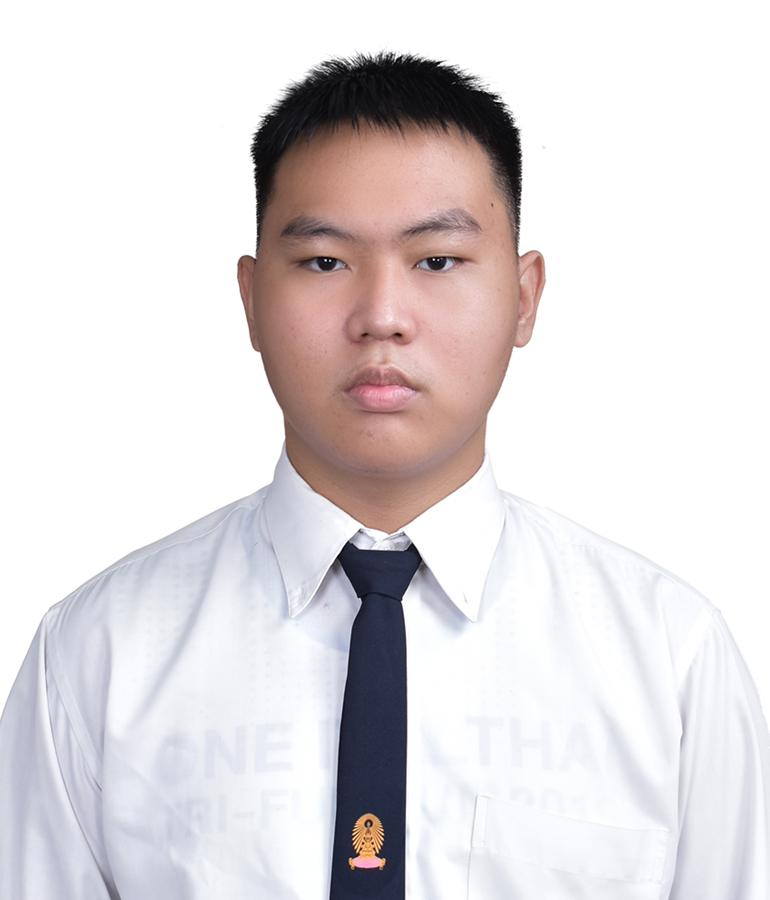
\includegraphics[width=0.75\linewidth]{image.jpg}
    \end{minipage}
    \par 

    \vspace{1em}

    \noindent
    \begin{minipage}{\textwidth}
        \large\textbf{Summary}\par
        \vspace{0.25em}
        \nointerlineskip
        \noindent
        \rule{0.25\textwidth}{0.4pt}
        \par

        \vspace{0.45em}
        \begin{minipage}{\textwidth}
            \normalsize
            \begingroup
            Software Engineer with a background in fullstack systems, VR research, and internal developer tooling.
            Values craftsmanship and thoughtful system design, with a focus on building reliable, impactful technology.
            \endgroup
        \end{minipage}
    \end{minipage}

    \vspace{0.85em}

    \noindent
    \begin{minipage}{\textwidth}
        \large\textbf{Experience}\par
        \vspace{0.25em}
        \nointerlineskip
        \noindent
        \rule{0.25\textwidth}{0.4pt}
        \par

        \vspace{0.45em}
        \begin{minipage}{0.595\textwidth}
            \normalsize
            \begingroup
                Software Engineer\par
                \textbf{Immersive Technology Lab of Chulalongkorn University}\par
            \endgroup
        \end{minipage}
        \hfill
        \begin{minipage}{0.255\textwidth}
            \normalsize
            \begingroup
            November 2023 - March 2025
            \endgroup
        \end{minipage}

        \vspace{0.35em}
        \hspace{0.1em}
        \begin{minipage}{0.99\textwidth}
            \normalsize
            \begingroup
            - \hspace{0.5em} Developed and conducted research on a transaction system for a Metaverse application, focusing on scalability and efficient data management.\par
            - \hspace{0.5em} Led a research team on stroke treatment using Virtual Reality, creating innovative solutions for therapeutic environments.\par
            - \hspace{0.5em} Compiled technical reports for paper writing, contributing to academic and industry publications.\par
            - \hspace{0.5em} Facilitated communication between the technical team and business stakeholders to align project goals and ensure smooth delivery.\par
            \endgroup
        \end{minipage}

        \vspace{0.85em}

        \begin{minipage}{0.725\textwidth}
            \normalsize
            \begingroup
                Back-end Developer Intern\par
                \textbf{Botnoi Group}\par
            \endgroup
        \end{minipage}
        \hfill
        \begin{minipage}{0.185\textwidth}
            \normalsize
            \begingroup
            May 2025 - July 2025
            \endgroup
        \end{minipage}

        \vspace{0.35em}
        \hspace{0.1em}
        \begin{minipage}{0.99\textwidth}
            \normalsize
            \begingroup
            - \hspace{0.5em} Trained new members to full productivity within one week of onboarding.\par
            - \hspace{0.5em} Developed AWS containerized services integrated with external vendor servers.\par
            - \hspace{0.5em} Developed internal project management tools used across the company.\par
            \endgroup
        \end{minipage}
    \end{minipage}

    \vspace{0.85em}

    \noindent
    \begin{minipage}{\textwidth}
        \large\textbf{Projects}\par
        \vspace{0.25em}
        \nointerlineskip
        \noindent
        \rule{0.25\textwidth}{0.4pt}
        \par

        \vspace{0.45em}

        \begin{minipage}{0.85\textwidth}
            \normalsize
            \begingroup
                Typescript\par
                \textbf{Form to docx}\par
            \endgroup
        \end{minipage}
        \hfill
        \begin{minipage}{0.04\textwidth}
            \normalsize
            \begingroup
            2023
            \endgroup
        \end{minipage}

        \vspace{0.35em}
        \begin{minipage}{0.993\textwidth}
            \normalsize
            \begingroup
            An automation tool which is used to read from Google Spreadsheet and generated the docx by given template which is being used for student filing a university's form.
            \endgroup
        \end{minipage}

        \vspace{0.85em}

        \begin{minipage}{0.85\textwidth}
            \normalsize
            \begingroup
                Typescript\par
                \textbf{CardEditor}\par
            \endgroup
        \end{minipage}
        \hfill
        \begin{minipage}{0.04\textwidth}
            \normalsize
            \begingroup
            2023
            \endgroup
        \end{minipage}

        \vspace{0.35em}
        \begin{minipage}{0.993\textwidth}
            \normalsize
            \begingroup
            A card creation tool for a custom card game which is use for both game designing and deck designing.
            \endgroup
        \end{minipage}

        %\vspace{0.85em}
        %\begin{minipage}{0.85\textwidth}
        %    \normalsize
        %    \begingroup
        %        Javascript\par
        %        \textbf{WebXR-Stroke-Helper}\par
        %    \endgroup
        %\end{minipage}
        %\hfill
        %\begin{minipage}{0.04\textwidth}
        %    \normalsize
        %    \begingroup
        %    2024
        %    \endgroup
        %\end{minipage}

        %\vspace{0.35em}
        %\begin{minipage}{0.993\textwidth}
        %    \normalsize
        %    \begingroup
        %    Created for stroke patient to recover from arm and hand disabilty. It is a WebXR application that can be used in VR headsets. It is a simple game that uses hand tracking to detect the movement of the hand and the arm. The game is designed to help stroke patients to recover from their disability by using their hand and arm in a fun way.
        %    \endgroup
        %\end{minipage}

        \vspace{0.85em}

        \begin{minipage}{0.85\textwidth}
            \normalsize
            \begingroup
                Go\par
                \textbf{Nakudynamo}\par
            \endgroup
        \end{minipage}
        \hfill
        \begin{minipage}{0.04\textwidth}
            \normalsize
            \begingroup
            2025
            \endgroup
        \end{minipage}

        \vspace{0.35em}
        \begin{minipage}{0.993\textwidth}
            \normalsize
            \begingroup
            Local DynamoDB runner which is also manage it's own dependency which leads to easier development setup.
            \endgroup
        \end{minipage}

        \vspace{0.85em}
        \begin{minipage}{0.993\textwidth}
            \normalsize
            \begingroup
            Other ongoing projects include a custom game engine, a personal CMS-backed blog platform, and an experimental Turing-complete programming language with C interoperability.
            \endgroup
        \end{minipage}
    \end{minipage}

    \vspace{0.85em}

    \noindent
    \begin{minipage}{\textwidth}
        \large\textbf{Publications}\par
        \vspace{0.25em}
        \nointerlineskip
        \noindent
        \rule{0.25\textwidth}{0.4pt}
        \par

        \vspace{0.45em}
        \begin{minipage}{0.85\textwidth}
            \normalsize
            \begingroup
                International Academy of Astronautics\par
                (Mission Idea Contest 7 Finalist)\par
                \textbf{ILNSS: Network for Position on Lunar Surface and Interplanetary Prototype}\par
            \endgroup
        \end{minipage}
        \hfill
        \begin{minipage}{0.04\textwidth}
            \normalsize
            \begingroup
            2021
            \endgroup
        \end{minipage}

        \vspace{0.35em}
        \hspace{0.1em}
        \begin{minipage}{0.99\textwidth}
            \normalsize
            \begingroup
            - \hspace{0.5em} Developed simulation models for satellite orbital movement using GNU Octave.\par
            - \hspace{0.5em} Implemented time dilation and radio signal intensity calculations for interplanetary communication.\par
            - \hspace{0.5em} Contributed to system-level design and feasibility analysis of the lunar navigation network.\par
            \endgroup
        \end{minipage}
    \end{minipage}

    \vspace{0.85em}

    \noindent
    \begin{minipage}{\textwidth}
        \large\textbf{Leaderships}\par
        \vspace{0.25em}
        \nointerlineskip
        \noindent
        \rule{0.25\textwidth}{0.4pt}
        \par

        \vspace{0.45em}
        \begin{minipage}{0.55\textwidth}
            \normalsize
            \begingroup
                Student Council of Chulalongkorn University\par
                Commissioner on One Stop Service\par
                \textbf{Leader}\par
            \endgroup
        \end{minipage}
        \hfill
        \begin{minipage}{0.10\textwidth}
            \normalsize
            \begingroup
            2022 - 2023
            \endgroup
        \end{minipage}

        \vspace{0.35em}
        \hspace{0.1em}
        \begin{minipage}{0.99\textwidth}
            \normalsize
            \begingroup
            - \hspace{0.5em} Adjust working system within commissioner section which lead to better workflow.\par
            - \hspace{0.5em} Provided technical support for council decision-making process.\par
            - \hspace{0.5em} Retrieving university club's data which lead to more centralize information that still uses today.\par
            \endgroup
        \end{minipage}

        \vspace{1em}

        \begin{minipage}{0.55\textwidth}
            \normalsize
            \begingroup
                Game Research and Development Club\par
                \textbf{Club President}\par
            \endgroup
        \end{minipage}
        \hfill
        \begin{minipage}{0.10\textwidth}
            \normalsize
            \begingroup
            2023 - 2024
            \endgroup
        \end{minipage}

        \vspace{0.35em}
        \hspace{0.1em}
        \begin{minipage}{0.99\textwidth}
            \normalsize
            \begingroup
            - \hspace{0.5em} Initialized Monthly Game Jam within a club which led to more interaction with broader Game Development Community.\par
            - \hspace{0.5em} Pushing club member who interested in game development to compete on Talent Showcase by Thailand Game Association.\par
            - \hspace{0.5em} Leading role on First Intania Tech Month event which leads to new culture on faculty that still going to this day.\par
            \endgroup
        \end{minipage}

        \vspace{1em}

        \begin{minipage}{0.55\textwidth}
            \normalsize
            \begingroup
                StoryTeller Team\par
                \textbf{Director/Music Composer}\par
            \endgroup
        \end{minipage}
        \hfill
        \begin{minipage}{0.125\textwidth}
            \normalsize
            \begingroup
            2024 - Present
            \endgroup
        \end{minipage}

        \vspace{0.25em}
        \hspace{0.1em}
        \begin{minipage}{0.99\textwidth}
            \normalsize
            \begingroup
            - \hspace{0.5em} Led creative direction and original composition for multiple team submissions to THE BMS OF FIGHTERS.\par
            - \hspace{0.5em} Collaborated with arrangers, vocalists, and visual artists to produce cohesive multi-track BMS submissions.\par
            - \hspace{0.5em} Contributed to team strategy and scoring optimization, resulting in competitive placements in international BMS music events.\par
            \endgroup
        \end{minipage}
    \end{minipage}

    \vspace{0.85em}

    \noindent
    \begin{minipage}{\textwidth}
        \large\textbf{Skills}\par
        \vspace{0.25em}
        \nointerlineskip
        \noindent
        \rule{0.25\textwidth}{0.4pt}
        \par

        \vspace{0.75em}
        \hspace{2em}
        \begin{minipage}{0.40\textwidth}
            \normalsize
            \begingroup
            - \hspace{1em} C\par
            - \hspace{1em} C++\par
            - \hspace{1em} Go\par
            - \hspace{1em} C\#\par
            \endgroup
        \end{minipage}
        \hfill
        \begin{minipage}{0.50\textwidth}
            \normalsize
            \begingroup
            - \hspace{1em} Java\par
            - \hspace{1em} Rust\par
            - \hspace{1em} Python\par
            - \hspace{1em} Javascript/Typecript\par
            \endgroup
        \end{minipage}
    \end{minipage}

    \vspace{0.85em}

    \noindent
    \begin{minipage}{\textwidth}
        \large\textbf{Tools}\par
        \vspace{0.25em}
        \nointerlineskip
        \noindent
        \rule{0.25\textwidth}{0.4pt}
        \par

        \vspace{0.75em}
        \hspace{2em}
        \begin{minipage}{0.40\textwidth}
            \normalsize
            \begingroup
            - \hspace{1em} FastAPI\par
            - \hspace{1em} GoFiber\par
            - \hspace{1em} MongoDB\par
            - \hspace{1em} Apache Kafka\par
            \endgroup
        \end{minipage}
        \hfill
        \begin{minipage}{0.50\textwidth}
            \normalsize
            \begingroup
            - \hspace{1em} ReactJS\par
            - \hspace{1em} AstroJS\par
            - \hspace{1em} Angular\par
            - \hspace{1em} Docker\par
            \endgroup
        \end{minipage}
    \end{minipage}

    \vspace{0.85em}

    \noindent
    \begin{minipage}{\textwidth}
        \large\textbf{Education}\par
        \vspace{0.25em}
        \nointerlineskip
        \noindent
        \rule{0.25\textwidth}{0.4pt}
        \par

        \vspace{0.75em}
        \hspace{2em}
        \begin{minipage}{0.45\textwidth}
            \normalsize{Bachelor of Engineering}\par
            \normalsize{Computer Engineering}\par
            \normalsize\textbf{Chulalongkorn University}\par
            \vspace{0.125em}
            \footnotesize{GPA 3.04}\par
        \end{minipage}
        \hfill
        \begin{minipage}{0.20\textwidth}
            \normalsize{August 2022 - Present}\par
        \end{minipage}
    \end{minipage}
\end{document}
